%                                                                 aa.dem
% AA vers. 8.2, LaTeX class for Astronomy & Astrophysics
% demonstration file
%                                                       (c) EDP Sciences
%-----------------------------------------------------------------------
%
%\documentclass[referee]{aa} % for a referee version
%\documentclass[onecolumn]{aa} % for a paper on 1 column  
%\documentclass[longauth]{aa} % for the long lists of affiliations 
%\documentclass[rnote]{aa} % for the research notes
%\documentclass[letter]{aa} % for the letters 
%\documentclass[bibyear]{aa} % if the references are not structured 
% according to the author-year natbib style

%
\documentclass[referee]{aa}  
\usepackage{natbib}
\bibpunct{(}{)}{;}{a}{}{,} % to follow the A&A style

%
\usepackage{graphicx}
%%%%%%%%%%%%%%%%%%%%%%%%%%%%%%%%%%%%%%%%
\usepackage{txfonts}
%%%%%%%%%%%%%%%%%%%%%%%%%%%%%%%%%%%%%%%%
%\usepackage[options]{hyperref}
% To add links in your PDF file, use the package "hyperref"
% with options according to your LaTeX or PDFLaTeX drivers.
%
\begin{document} 


   \title{JUICE-ExPRES}

   \subtitle{}

   \author{B. Cecconi
          \inst{1}
          \and
          C. Louis\inst{2}
          }

   \institute{LESIA, Observatoire de Paris, CNRS, PSL Research University, Meudon, France\\
              \email{baptiste.Cecconi@observatoiredeparis.psl.eu}
         \and
             IRAP, CNRS, Université Paul Sabatier, Toulouse, France\\
             \email{corentin.louis@irap.omp.eu}
             }

   \date{}

% \abstract{}{}{}{}{} 
% 5 {} token are mandatory
 
  \abstract
  % context heading (optional)
  % {} leave it empty if necessary  
   {}
  % aims heading (mandatory)
   {Validate the use of ExPRES as an observation planning tool for the JUICE mission.}
  % methods heading (mandatory)
   {We simulate the occultations of the Jovian auroral radio emissions during the Galileo flybys of the Galilean moons of Jupiter. The ExPRES simulations runs are configured using fixed typical parameters for the main aurora radio emissions. We compare the simulation run results with the actual Galileo PWS observations.}
  % results heading (mandatory)
   {The ExPRES code accurately models the temporal occurrence of the occultations in the whole spectral range observed by Galileo PWS.}
  % conclusions heading (optional), leave it empty if necessary 
   {}

   \keywords{Radio emissions --
                Jupiter -- 
                JUICE mission
               }

   \maketitle
%
%________________________________________________________________

\section{Introduction}

The Jovian radio emissions

Galileo 

JUICE 

ExPRES \citep{Louis_AA_2019}   

%__________________________________________________________________

\section{Jovian radio emissions occultations}

As showed in \citet{Kurth:1997in}, the Jovian hectometric radio emissions are occulted by Ganymede during G01 flyby (Ganymede flyby during the first orbit around Jupiter) of the Galileo spacecraft, on June 27th 1996. Figure \ref{fig:g01} shows the Galileo/PWS (Plasma Waves Science) \citep{gurnett_SSR_92} spectrogram during G01 flyby. The occultation is observed between 05:50 and 06:20 SCET. The occultation spectral ingress and egress profiles imply that radio sources at higher frequencies (located close to Jupiter) are occulted earlier and reappears later than the lower frequency sources (located further out from Jupiter).

\begin{figure}
\includegraphics[width=\linewidth]{gll-G01-Kurth97.png}
\caption{Galileo PWS spectrogram observed during G01 flyby. The Jovian radio emissions present in the hectometric spectral range (from $\sim$300 kHz to $\sim$5 MHz). The occultation is labeled on the figure. Figure extracted from \citet{Kurth:1997in}.}\label{fig:g01}
\end{figure}

Occultations of the Jovian radio emissions have been also reported during the first Io flyby of Galileo \citep{louarn_GRL_97}. Figure \ref{fig:flyby_data} shows  Galileo/PWS observations of clear occultation of the Jovian radio emissions for each Galilean moon.

\begin{figure}
    \centering
    \includegraphics[width=0.49\linewidth]{gll-I24-das2.png}
    \includegraphics[width=0.49\linewidth]{gll-E12-das2.png}
    \includegraphics[width=0.49\linewidth]{gll-G01-das2.png}
    \includegraphics[width=0.49\linewidth]{gll-C30-das2.png}
    \caption{Jovian radio emission occultations by Io (upper left), Europa (upper right), Ganymede (lower left) and Callisto (lower right).}
    \label{fig:flyby_data}
\end{figure}

\section{Radio occultation modeling}

We model the location of the Jovian auroral radio sources visible at Galileo's location using ExPRES (Exoplanetary and Planetary Radio Emission Simulator) \citep{Louis_AA_2019}. The location of the visible radio sources is modeled every minute of time during the interval displayed on Figure \ref{fig:g01}. Northern and Southern main auroral oval are modeled with active magnetic field lines every 1$^\circ$ in longitude.  We use the JRM09 magnetic field model \citep{Connerney:2018jx} and the magnetic latitude of the active magnetic field lines corresponds to $L_\textrm{shell}=30$ \citep{Grodent:2015eo}. The unstable electron temperature set to 5~keV \citep{Louarn:2017bc}. These parameters are typical parameters and are fixed for all simulation runs used in this study.

The occultation itseft is computed using a simple derivation of the intercept distance between the center of the Galilean moon and the straight lines passing by each visible modelled radio source and the observer. Any source with an intercept distance shorter than one moon radius is occulted, as sketched on Figure \ref{fig:occult}.

When the observer is located near the magnetic equator, the radio source beaming pattern implies that the radio visible radio source can be split into four classes, called A, B, C and D, corresponding respectively to the North-Eastern, North-Western, South-Eastern and South-Western quadrant around Jupiter as seen from the observer \citep[see, e.g.,][for a definition]{Louis_AA_2019}. 

%The second occultation estimation includes a model of the Ganymede's ionosphere (e.g., as in Eviatar et al (2001)), and uses the modeled cutoff frequency altitude for each frequency.

\begin{figure}
\centering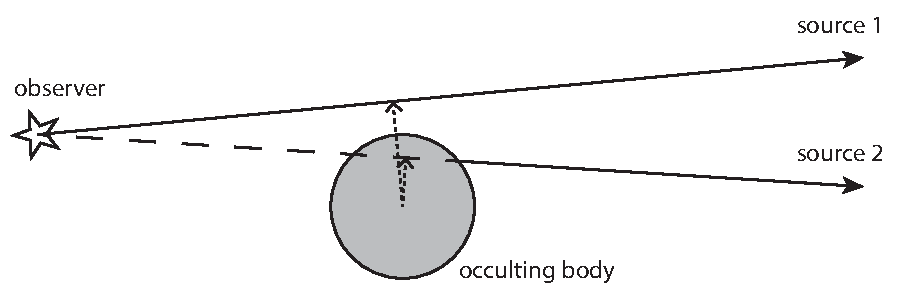
\includegraphics[width=0.7\linewidth]{occult.pdf}
\caption{Simple geometrical occultation scheme used in this study. The intercept distance (dotted segment) is computed as the distance between the center of occulting moon, and the straight line passing by each radio source and the observer.}\label{fig:occult}
\end{figure}

\section{Datasets}
All Galilean moon flyby of Galileo with PWS data have been modelled and analyzed. The GLL/PWS data have been retrieved from University of Iowa das2 server interface \cite{piker_2019}.  

ExPRES simulation runs have been processed using the online interface described in \citet{Louis_AA_2019}. 


\section{Results}
The comparison of observed and modelled data shows that Europa, Ganymede, and Callisto occultations are modeled with a one minute accuracy. 

\section{Discussion}

\section{Conclusions and Perspectives}

Further analysis with ionosphere model of Galilean moons.

\section*{Acknowledgments}

\bibliographystyle{aa}
\bibliography{juice-expres}
\end{document}
